\documentclass[12pt]{article}

\usepackage{fixltx2e}
\usepackage{textcomp}
\usepackage{fullpage}
\usepackage{amsfonts}
\usepackage{verbatim}
\usepackage[english]{babel}
\usepackage{pifont}
\usepackage{color}
\usepackage{setspace}
\usepackage{lscape}
\usepackage{indentfirst}
\usepackage[normalem]{ulem}
\usepackage{booktabs}
% \usepackage{nag}
\usepackage{natbib}
% \usepackage{bibtex}
\usepackage{float}
\usepackage{latexsym}
\usepackage{hyperref}
\usepackage{url}
% \usepackage{html}
\usepackage{epsfig}
\usepackage{graphicx}
\usepackage{amssymb}
\usepackage{amsmath}
\usepackage{bm}
\usepackage{array}
%\usepackage{mhchem}
\usepackage{ifthen}
\usepackage{caption}
\usepackage{xcolor}
\usepackage{amsthm}
\usepackage{amstext}
\usepackage{nicefrac}
\usepackage{algorithm}
\usepackage{algorithmic}
\usepackage[scientific-notation=true]{siunitx}
\usepackage{subfigure}
\usepackage[flushleft]{threeparttable}
\usepackage{lineno}
\usepackage{adjustbox}

%Rename figure or table label number
\renewcommand{\thefigure}{S\arabic{figure}}
\renewcommand{\thetable}{S\arabic{table}}

\begin{document}

\begin{minipage}[h]{\textwidth}
	\title{Supplementary information for StarBEAST2}
	\author{Huw A. Ogilvie$^{\ast,1,2}$ and Alexei J. Drummond,$^{2,3}$}
    \maketitle
\end{minipage}

\raggedright
$^{1}$Department of Evolution, Ecology and Genetics, Australian National University, Canberra, Australia\\
$^{2}$Centre for Computational Evolution, University of Auckland, Auckland, New Zealand\\
$^{3}$Department of Computer Science, University of Auckland, Auckland, New Zealand

\clearpage

\section{Validation of correctness}

\begin{figure}[htb!]
\centering
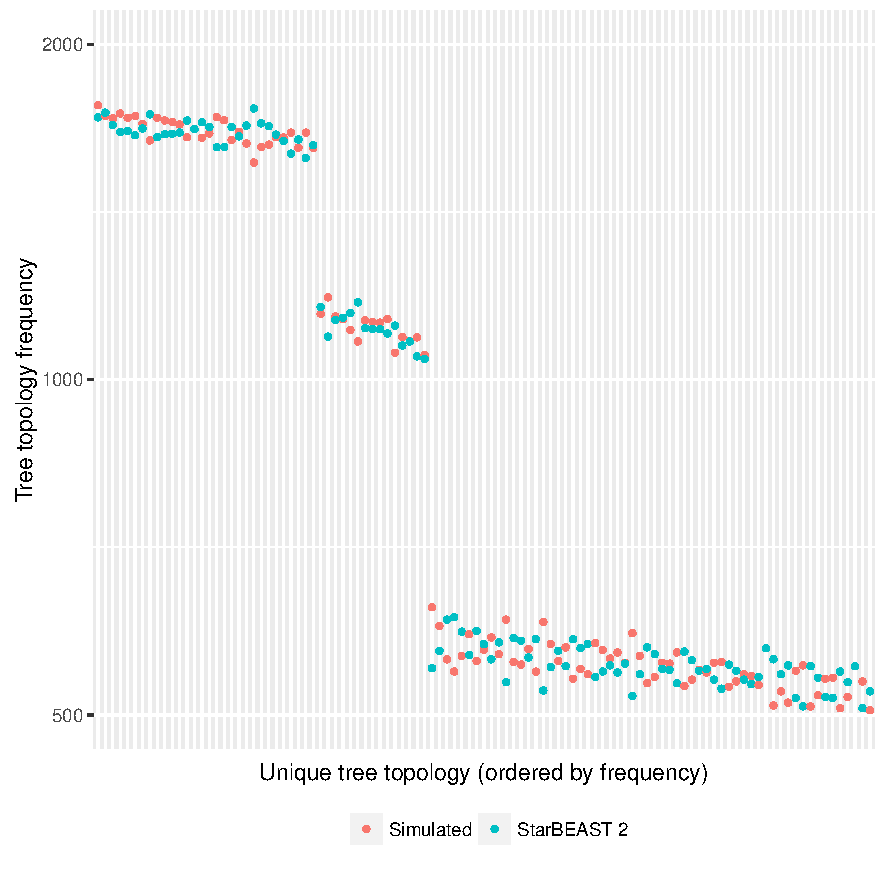
\includegraphics[width=16cm]{species_topology_frequencies.pdf}
\caption
{Frequency of five-taxon species tree topologies sampled from a birth-death prior
distribution. Topologies were sampled by simulating trees using biopy (red), or
by using a StarBEAST2 MCMC chain (blue). Frequencies are identical apart from
noise, indicating that StarBEAST2 is mathematically correct. Three levels of
probability are evident from left to right --- high probability balanced
topologies e.g. ((a,b),((c,d),e)), middle probability intermediate topologies
e.g. (((a,b),(c,d)),e), and low probability unbalanced topologies e.g.
((((a,b),c),d),e).}
\label{fig:speciesTopologyFrequencies}
\end{figure}

\clearpage

\begin{figure}[htb!]
\centering
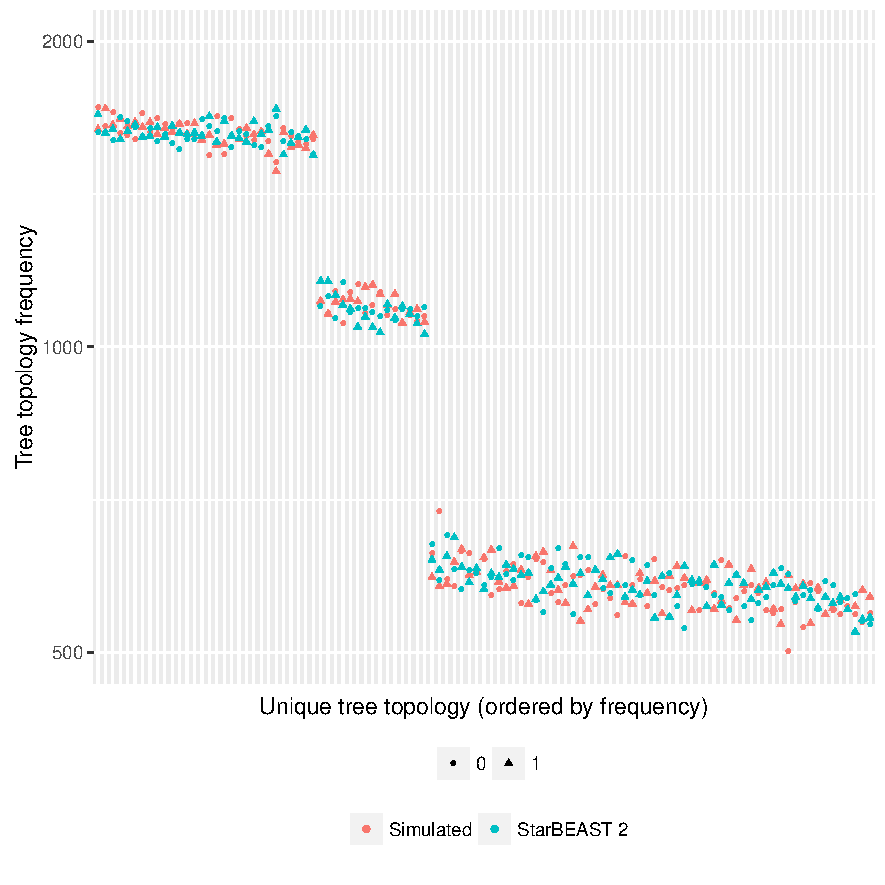
\includegraphics[width=16cm]{gene_topology_frequencies.pdf}
\caption
{Frequency of five-taxon gene tree topologies sampled from a multispecies coalescent prior
distribution. Topologies were sampled by simulating gene trees within species trees using biopy (red), or
by using a StarBEAST2 MCMC chain (blue). Frequencies are identical apart from
noise, indicating that StarBEAST2 is mathematically correct. Three levels of
probability are evident from left to right --- high probability balanced
topologies e.g. ((a,b),((c,d),e)), middle probability intermediate topologies
e.g. (((a,b),(c,d)),e), and low probability unbalanced topologies e.g.
((((a,b),c),d),e).}
\label{fig:geneTopologyFrequencies}
\end{figure}

\clearpage

\begin{figure}[htb!]
\centering
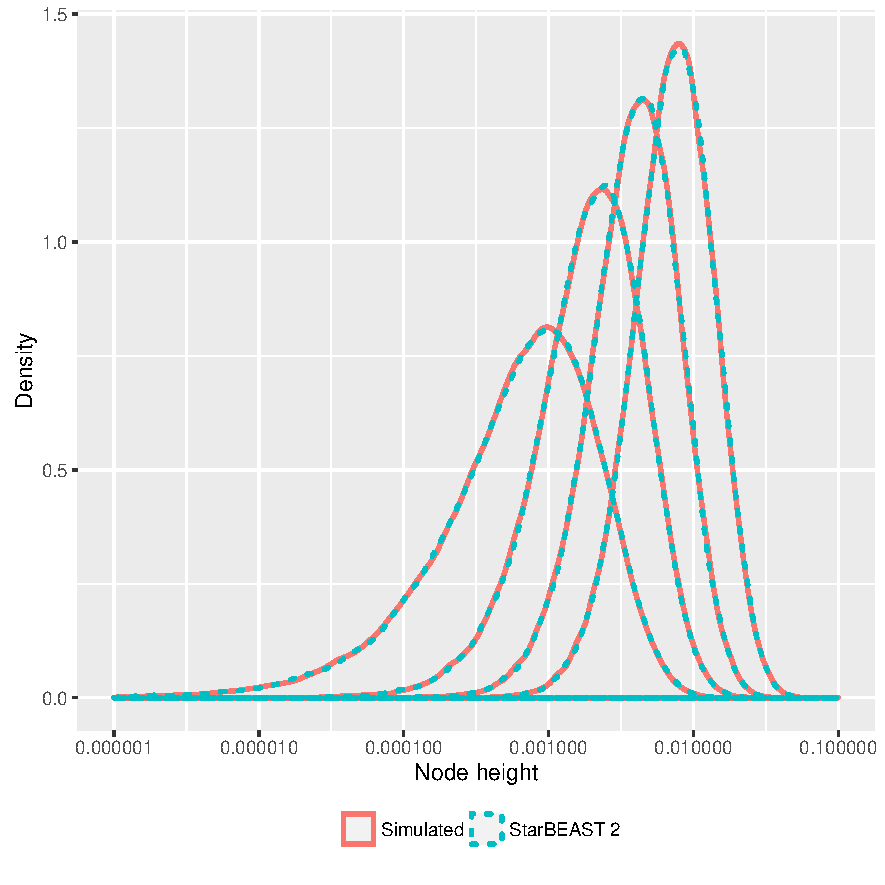
\includegraphics[width=16cm]{species_node_heights.pdf}
\caption
{Probability densities of five-taxon species tree node heights sampled from a
birth-death prior distribution. Node heights were sampled by simulating trees
using biopy (red), or by using a StarBEAST2 MCMC chain (blue). Probability
densities are plotted separately for each ranked node giving four peaks, one
for each internal node. Node height probability densities are identical apart
from noise, indicating that StarBEAST2 is mathematically correct.}
\label{fig:speciesNodeHeights}
\end{figure}

\clearpage

\begin{figure}[htb!]
\centering
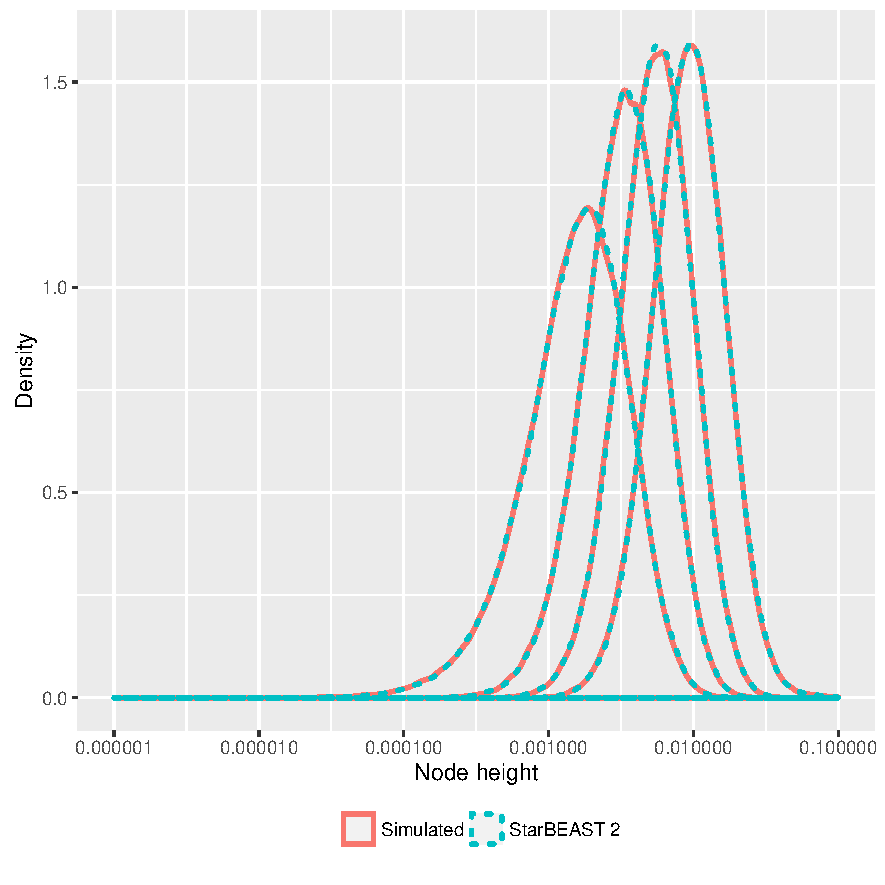
\includegraphics[width=16cm]{gene_node_heights.pdf}
\caption
{Probability densities of five-taxon gene tree node heights sampled from a
multispecies coalescent prior distribution. Node heights were sampled by simulating gene trees
within species trees using biopy (red), or by using a StarBEAST2 MCMC chain (blue). Probability
densities are plotted separately for each ranked node giving four peaks, one
for each internal node. Node height probability densities are identical apart
from noise, indicating that StarBEAST2 is mathematically correct.}
\label{fig:geneNodeHeights}
\end{figure}

\clearpage

\begin{figure}[htb!]
\centering
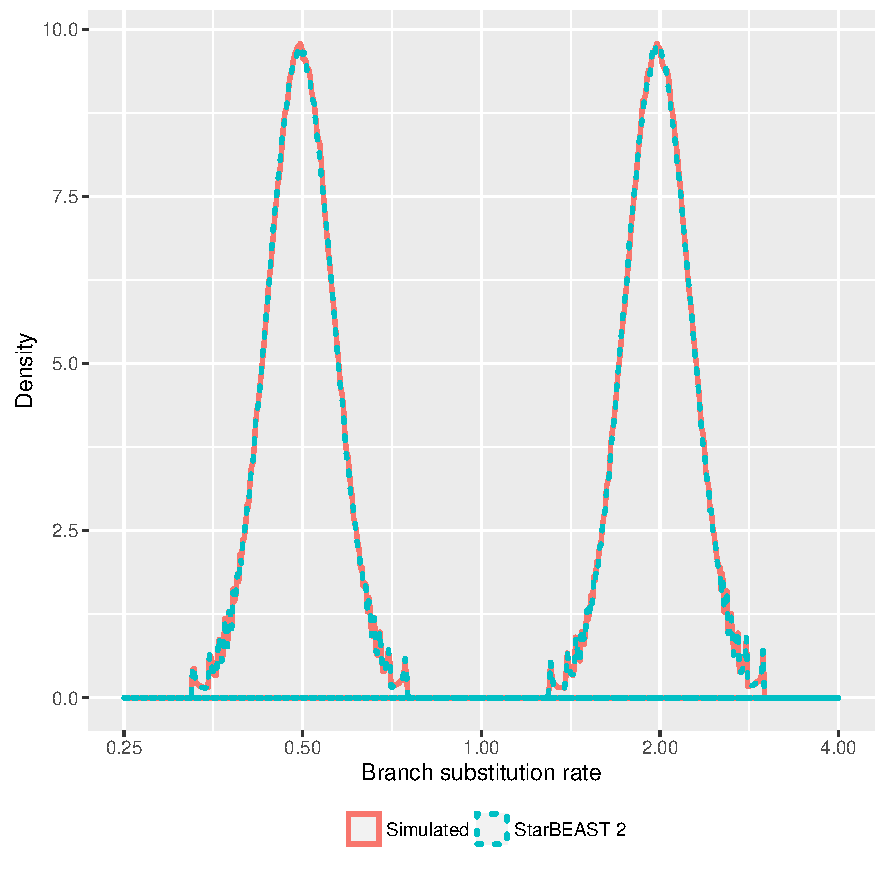
\includegraphics[width=16cm]{gene_branch_rates.pdf}
\caption
{Probability densities of five-taxon gene tree branch rates produced by a
species tree uncorrelated lognormal (UCLN) relaxed clock. Branch rates were
sampled by simulating gene trees within species trees using biopy and simulating
species tree branch rates using scipy (red), or by using a StarBEAST2 MCMC chain
(blue). Two lognormal distributions were used, one with a mean of 0.5 and the
other with a mean of 2.0, resulting in two peaks. Branch rate probability
densities are identical apart from noise, indicating that StarBEAST2 is
mathematically correct.}
\label{fig:geneBranchRates}
\end{figure}

\clearpage

\end{document}
